\documentclass[letterpaper,twocolumn,10pt]{article}
\usepackage{usenix2019,epsfig,endnotes}
\usepackage{slashbox}
\usepackage{algorithm}
\usepackage{algpseudocode}
\usepackage{url}
\usepackage{threeparttable}
\usepackage{color}

\usepackage{amsmath}
\usepackage{bm}
\usepackage{lettrine}
% \begin{document}

\renewcommand{\algorithmicrequire}{\textbf{Input:}}  % Use Input in the format of Algorithm
\renewcommand{\algorithmicensure}{\textbf{Output:}} % Use Output in the format of Algorithm

\newcommand{\psz}[1]{\textcolor{red}{\footnotesize [PSz: #1]}}
\newcommand{\bowen}[1]{\textcolor{blue}{\footnotesize [Bowen: #1]}}
\newcommand{\chunpeng}[1]{\textcolor{red}{\footnotesize [Chunpeng: #1]}}

\makeatletter\def\@captype{table}\makeatother

\begin{document}

\date{}

\title{\Large \bf Statistical Research On The Effective Relaxation}

%for single author (just remove % characters)
\author{
{\rm Xiaolong Feng}\\
xiaolong\_feng@mymail.sutd.edu.sg\\
SUTD, Singapore
\and
{\rm Yin Jia}\\
yin\_jia@mymail.sutd.edu.sg\\
SUTD, Singapore
\and
{\rm Bowen Liu}\\
bowen\_liu@mymail.sutd.edu.sg\\
SUTD, Singapore
\and
{\rm Guangtong Li}\\
guangtong\_li@mymail.sutd.edu.sg\\
SUTD, Singapore
\and
{\rm Wang Zhang}\\
wang\_zhang@mymail.sutd.edu.sg\\
SUTD, Singapore
}

\maketitle

\thispagestyle{empty}

\subsection*{Abstract}
There are significant differences in brain waves between people who are highly focused and those who are completely relaxed. We used the Electroencephalography (EEG) collector to measure the EEG of people in different environments, and use the data processing methods learned in the research method class to process and analyze the collected data, so as to find an efficient way for people to relax. The main steps include: Collecting the EEG signals, transforming the signals from time domain to frequency domain using Fast Fourier Transform (FFT), analyzing the signals in frequency domain using statistical methods such as one-way analysis of variance (ANOVA), Hotteling $T^2$ test and two-way ANOVA.


\textbf{Key words}: Electroencephalography (EEG) analysis, Fast Fourier Transform, One-way ANOVA, Hotteling $T^2$ test, Two-way ANOVA


\section{Introduction}

Electroencephalography (EEG) is one of the main tools in the practice of clinical neurology. Not withstanding the development of increasingly detection methods, including computed tomography (CT) scanning, magnetic resonance imaging (MRI), and nuclear medicine imaging, the use of EEG in the study of brain activities continues to increase. EEG captures electrical information over time. As CT and MRI do not give direct information regarding electrical irritability in the brain or even indicate whether the testee is awake or asleep, the electroencephalography is an important complementary technique for brain behavior study and has been widely studied.

For instance, Bartels G et al~\cite{bartels2010automatic}, studied and obtained an effective algorithm for removing artifacts in EEG signal pre-processing. Nie~\cite{nie2011eeg} discovered the main associated with emotional EEG signals generated by Gamma spectrum of left frontal and temporal lobe. Vijayan~\cite{vijayan2015eeg,bashar2015identification,torres2014comparative} introduced a novel approach towards classification of various human emotions based on statistically weighed autoregressive modelling of Electroencephalogram (EEG) signals. Abo-Zahhad~\cite{abo2015state} and Wei et al.~\cite{wei2015selective} discussed the employment of brain signals for human recognition tasks. Acharya~\cite{acharya2015novel} presented a novel method for automated EEG-based diagnosis of depression using nonlinear methods. Pachori~\cite{pachori2014epileptic} presented a new method for classification of ictal and seizure-free EEG signals. Riaz~\cite{riaz2016emd} presented the usage of up to third order temporal moments, and spectral features. Xu~\cite{xu20151} proposed a novel 1.5-D algorithm for multi-channel electroencephalogram (EEG) compression.

Though many works have been done in this area, there are still many issues that have not been intensively studied. In this project, we aim to analyze the influence of doing different activities on the change of brain waves and figure out the statistically significant factors,and find the most effective way for people in modern society to relax. Section 2 details the setup of the experiment; Section 3 introduces the statistical model used in this project; Section 4 analyses the measured data and discusses the results. Section 6 summarizes the entire project.

\section{Statistical Model}

\subsection{One-way ANOVA}
One factor analysis of variance~\cite{Anova} is a special case of analysis of variance (ANOVA), for one factor of interest, and a generalization of the two-sample t-test. For example, data collected on, say, five instruments have one factor (instruments) at five levels. The ANOVA tests whether instruments have a significant effect on the results and is used to test the degree to which two or more groups differ in an experiment.

To achieve this, we need to calculate the F-test which is used to compare whether two variances are similar. A small F-value may indicate that the sample variances are different. We can use it to test whether the groups differ from one. To perform one-way ANOVA, we also need to compute both the between-group variance and the in-group variance.

\subsection{Two-way ANOVA}
The two-way analysis of variance (two-way ANOVA) is an extension of the one-way ANOVA that examines the influence of two different categorical independent variables on one continuous dependent variable. Comparing to the one-way ANOVA, the two-way ANOVA not only study the main effect of each independent variable but also the interaction between them.

Let $A$ and $B$ be the two factors, the total variability is $SST=SSA+SSB+SSAB+SSE$, where $SSA$ quantifies the variability of factor $A$ due to factor $B$ changing, and $SSB$ is the variability of factor B due to changing of factor A. The total sum of squares can be calculated as $SST=\sum\limits_{i=1}^{a}\sum\limits_{j=1}^{b}\sum\limits_{k=1}^{n}\left( y_{ijk}-\left\langle y\right\rangle \right) ^2$, where $\left\langle y\right\rangle$ is the mean of all the responses, $a$ is the number of levels of factor A, $b$ is the levels of factor B, and $n$ is the number of replications per cell. $SSA$, $SSB$, $SSE$ can be calculated as $SSA=bn\sum\limits_{i=1}^{a}(\bar{A}_i- \left\langle y\right\rangle)^2$, $SSB=an\sum\limits_{j=1}^{b}(\bar{B}_i- \left\langle y\right\rangle)^2$, $SSE=\sum\limits_{i=1}^{a}\sum\limits_{j=1}^{b}\sum\limits_{k=1}^{n}(y_{ijk}-\bar{y}_{ij})^2$ respectively. Finally, we can calculate $SSAB$ as $SSAB=SST-SSA-SSB-SSE$. After obtaining the variabilities, the mean squares can be calculated as $MSA=\frac{SSA}{a-1},MSB=\frac{SSB}{b-1},MSAB=\frac{SSAB}{(a-1)(b-1)},MSE=\frac{SSE}{ab(n-1)}$ respectively. Then the F-test can be performed for each factor as $F_A=\frac{MSA}{MSE},F_B=\frac{MSB}{MSE},F_{AB}=\frac{MSAB}{MSE}$. If $F>F_c$, we could conclude that the factor has a significant influence on the response; if $F<F_c$, then the factor has no significant influence on the response.

\subsection{Hotteling $T^2$ Test}

Multivariate analysis deals with the statistical differences between samples of multiple different parameters. Multivariate Hotteling $T^2$ test was used for multivariate analysis in this project. Consider the t-statistic for univariate mean $t=\frac{\bar{x}-\mu}{s/\sqrt{n}}$, where $\bar{x}$ is the sample mean, $\mu$  is the population mean, $s$ is sample standard deviation, $n$ is the sample size, for $t^2$ we have $t^2=\frac{(\bar{x}-\mu)^2}{s^2/n}$. Thus the F-statistic is applicable and $H_0$ is rejected at significance level $\alpha$ if $t^2$ is greater than the critical value from the F-table. Rewriting $t^2$ we get $t^2=n(\bar{x}-\mu)\left( \frac{1}{s^2}\right) (\bar{x}-\mu)$, and it can be extended for a multivariate vector of means as $T^2=n(\bm{\bar{X}}-\mu)^T\bm{C}^{-1}(\bm{\bar{x}}-\mu)$, where $\bm{\bar{X}}$ is a vector of sample means, $\bm{C}^{-1}$ is a vector of the corresponding variance-covariance matrix, and $\mu$ is a vector of the corresponding population means. Overall, Hotelling $T^2$ test examines whether two multivariate datasets are significantly different.


\section{Experiment}
In this section, we discussed how we collected data and conducted data analysis.

All the data were collected in an isolated room which lights and power point(AC) were turn off to minimize the interference in Radio-Frequency. Because we found that there is an unexpected figure with 50Hz appearred in generated data if the AC and lights were powered on.

To evaluate the factors on emotion, we collected the data in four main parts.

\noindent
\hangafter=1
\setlength{\hangindent}{1em}
\textbf{Music}: we statistically collected the brain wave when testee listened to the music without any interference. To achieve this, testee was requested to listen music with eye closed and stay in the calm state. In total, we selected three music categories which are Always with me(light music,the theme song in the movie of Spirited Away) , 2014 World Cup theme song(rock music) and Yesterday once more(pop music) respectively.

\noindent
\hangafter=1
\setlength{\hangindent}{1em}
\textbf{Game}: is always a relaxing activity when you want to release stress. Three popular games were selected which are Player Unknown’s Battlegrounds(competitive game), Anipop(casual game) and Poker Game(mind sports).

\noindent
\hangafter=1
\setlength{\hangindent}{1em}
\textbf{Movie}: can measure the brain wave of testee from visual sense. Three categories were selected which are Agent Mr. Bean (Comedy), Japanese, Ju-on: The Grudge(Horrible movie) and About Time(Touching movie).

\noindent
\hangafter=1
\setlength{\hangindent}{1em}
\textbf{Two-Factor}: is used for two-factor ANOVA analysis. We simply showed the results by collecting testee's data when he listened to music while playing games. Each factor has two levels therefore there are four circumstances (light music with casual game, light music with competitive game, rock music with casual game, rock music with competitive game)

The aim of data collection goes to three parts. One is for Hotteling $T^2$ Test which tests whether two multivariate datasets are significantly different. The other is for one-factor ANOVA which we measured totally nine vectors to obtain results and last one is for two-factor ANOVA.

Moreover, we tested the participant in the relaxing and peaceful status. For brain wave, we analysized the frequency of wave from different five scope, ranging from 0.5-4Hz(Delta), 4.0-8.0Hz(Theta), 8.0-13.0Hz(Alpha), 13.0-30.0(Beta) and 30.0-45.0Hz(Gamma). We simply showed the figure for the horrible movies brain waves in Figure 1.
% \begin{figure}[t]
% \begin{picture}(300,150)(-10,30)
%   \centering
%   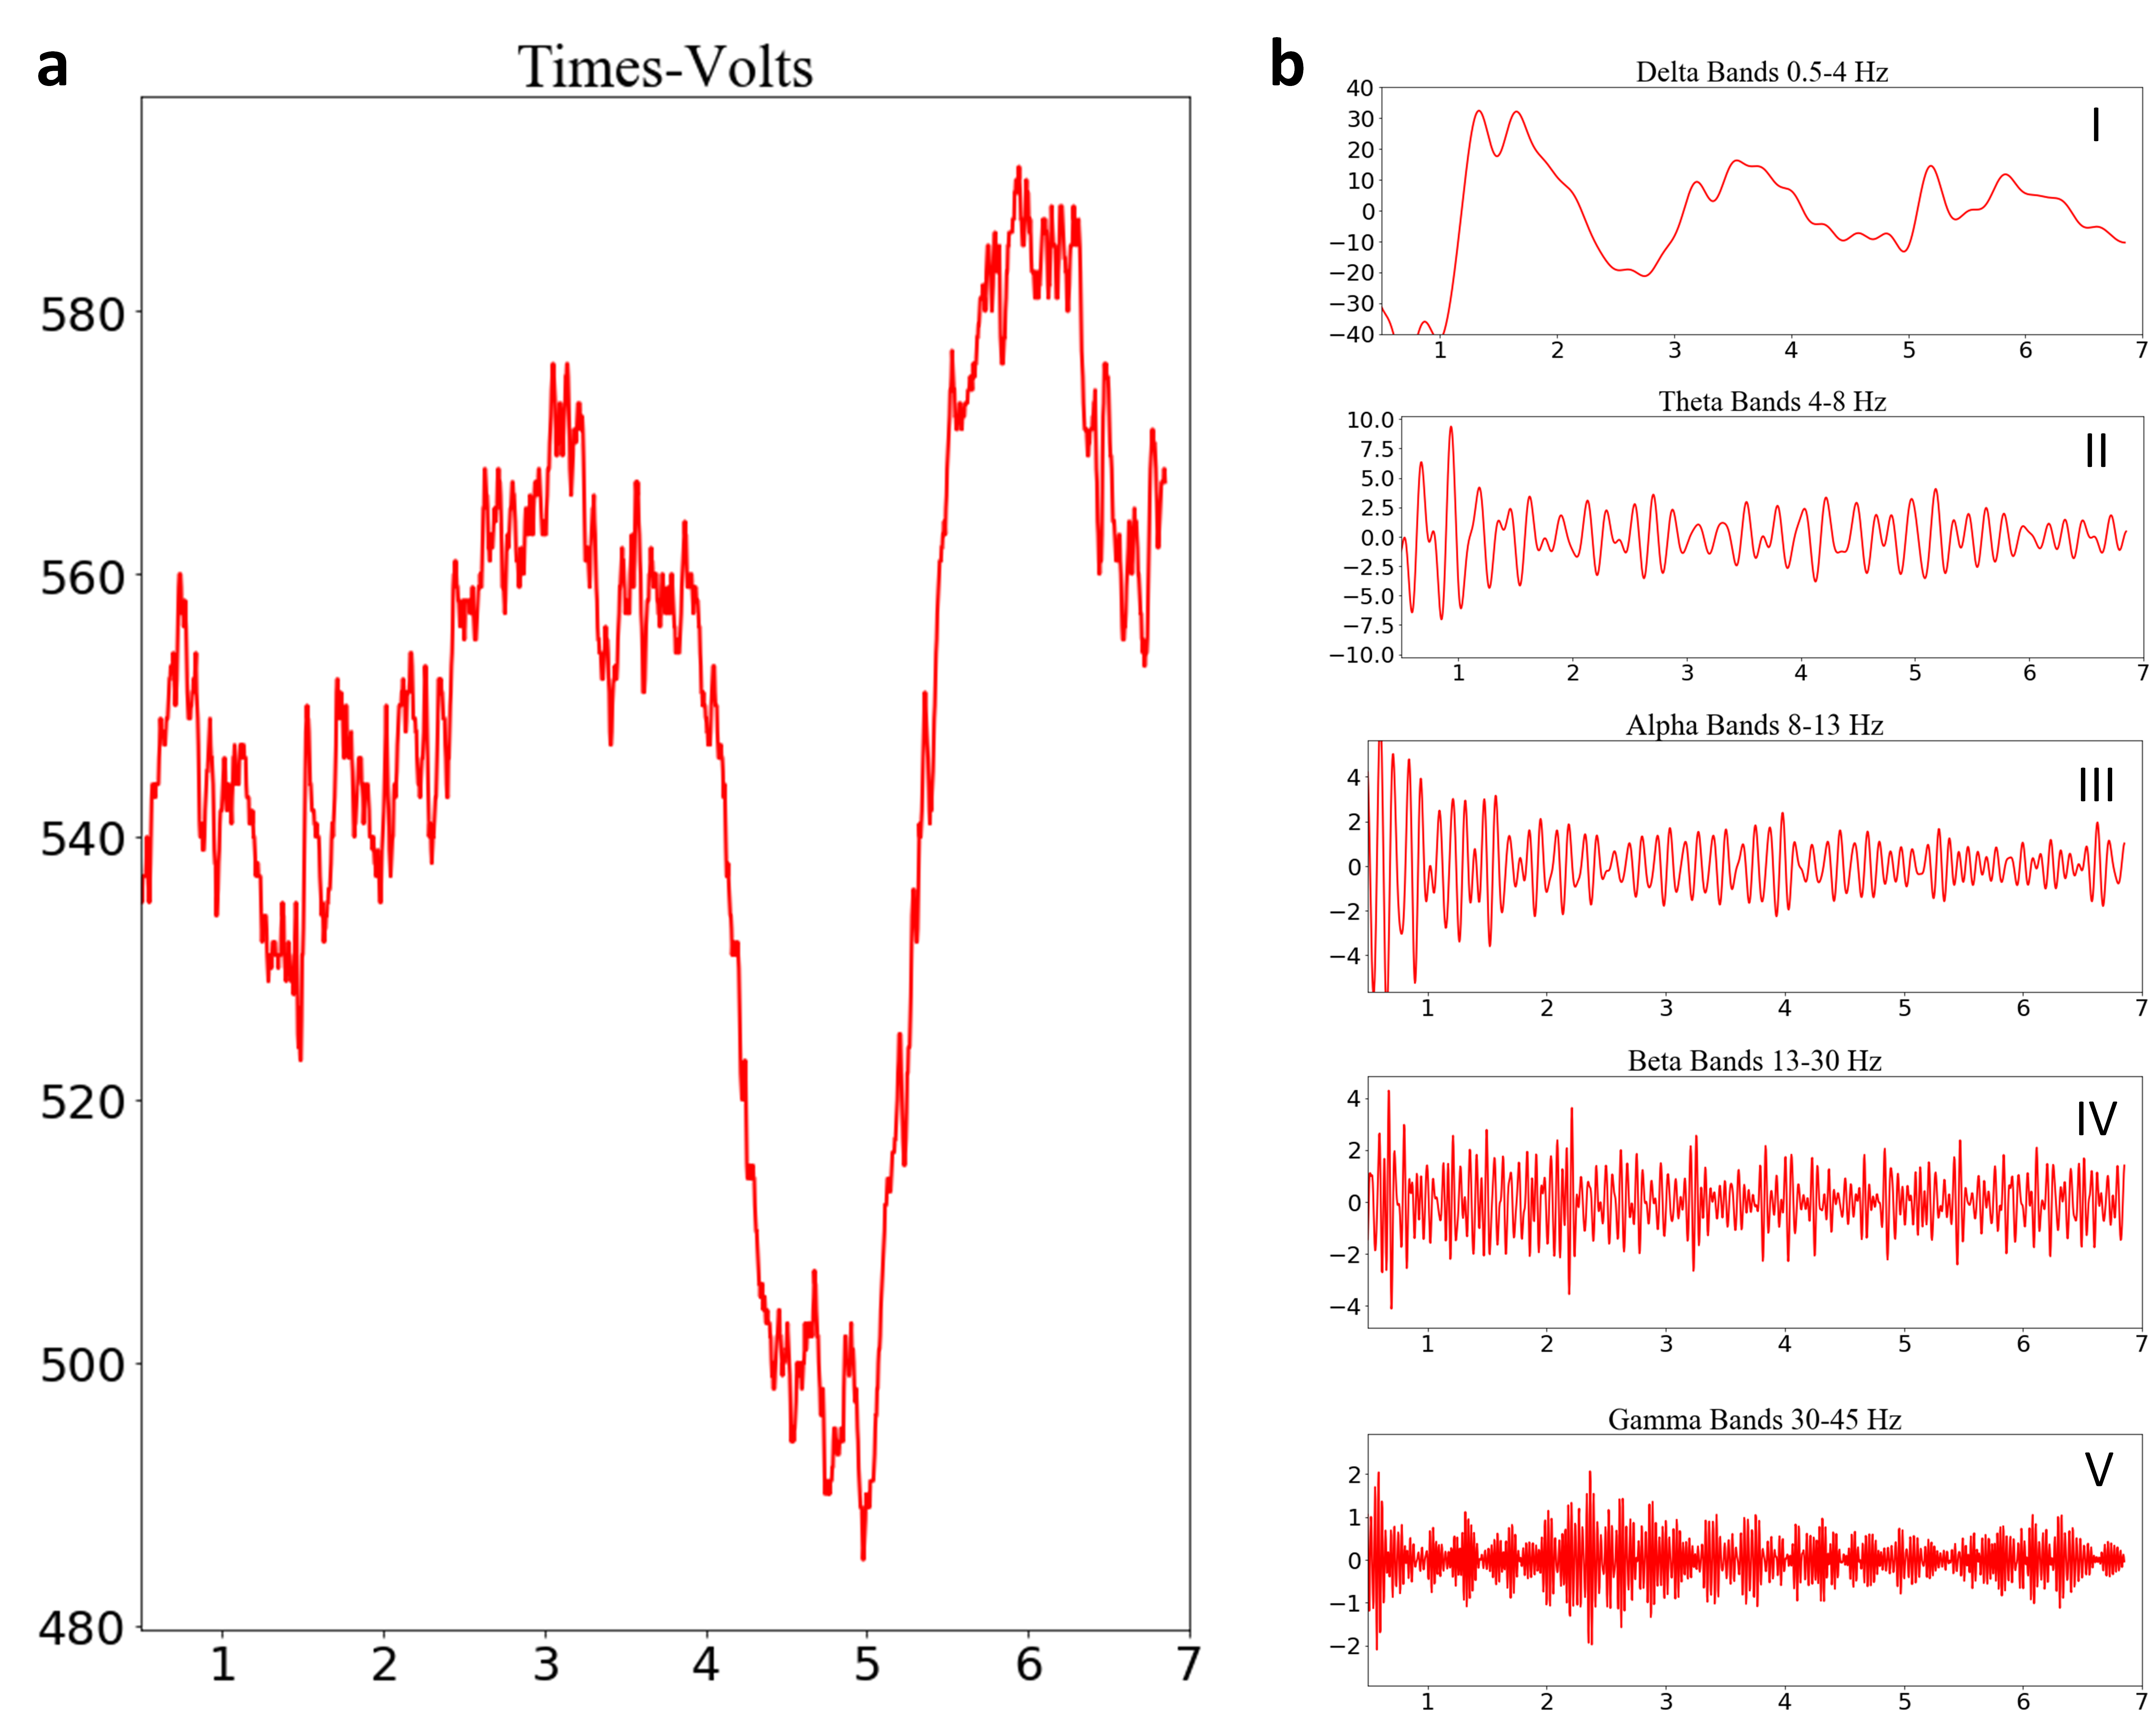
\includegraphics[width=0.8\linewidth]{fig/waves}
%   \put(-15,-30){\special{psfile = fig1.ps hscale = 100 vscale = 100}}
% \end{picture}\\
%   \caption{Frequency range for horrible movie activity}
%   \label{fig:waves}
% \end{figure}

\begin{figure*}[h!]
  \centering
  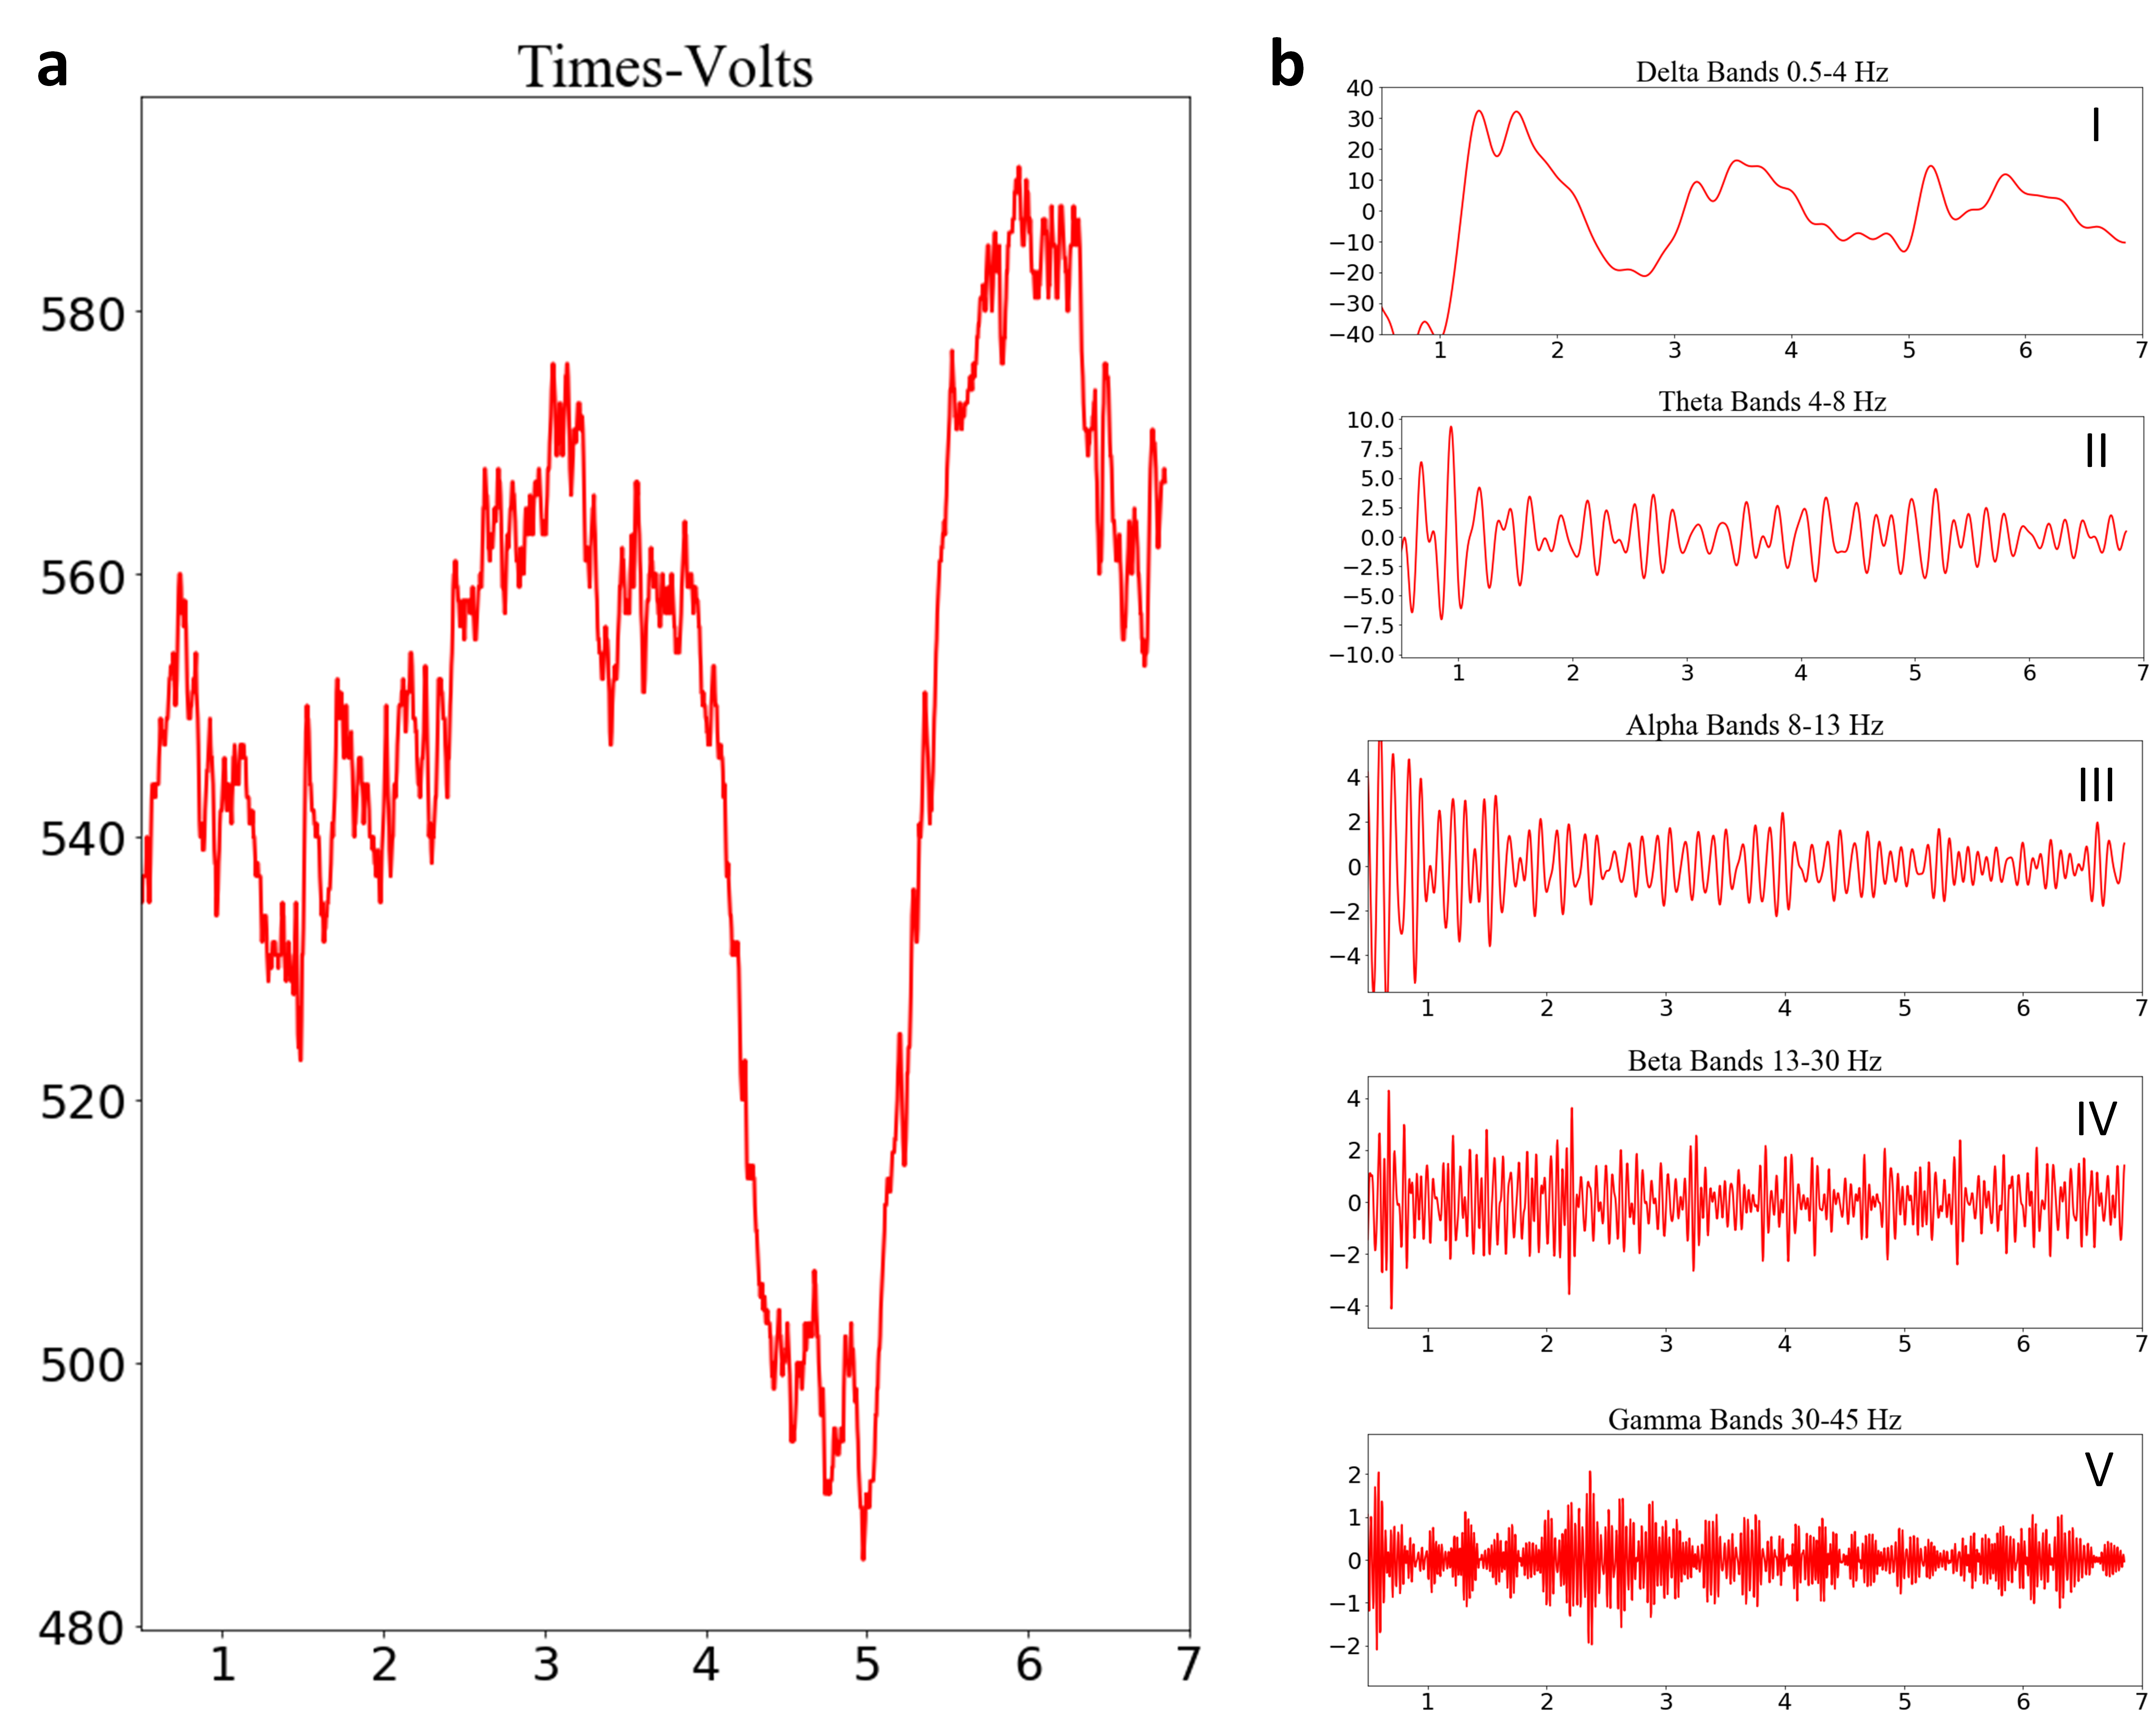
\includegraphics[width=0.8\linewidth]{fig/waves}
  \caption{Five typical brain rhythms (b) extracted from the measured EEG signal (a) when watching horrible movie.}
  \label{fig:waves}
\end{figure*}


\section{Analysis and Evaluation}
In this section, we will discuss the statistic analysis methods whihc we leveraged on the collected data and how we evaluated our analysis results.

\subsection{One-way ANOVA}

The format of collected data contains two fields: time and volts. For the convenience of analysis, we firstly extracted the two-column data by using pandas package in Python. Then, we could get the amplitude list after using FFT function. As discussed above, the whole result contains totally five frequencies (Delta, Theta, Alpha, Beta, Gamma). Therefore, we extracted from each range and there are nine vectors in each range as each vector represents one activity shown in \ref{fig:one-1} .

In our experiments, we collected 15 samples in total for each category and for precise purpose we chose ten of all samples from each categories and calculated the mean of amplitude in each sample. The rule of how to choose 10 out of 15 samples is that we wrote an algorithm to find the closest 10 data among the number of 15 data.

After extracting data from native collected data completely, we wrote the function to calculate the F-value for each groups. There are 5 groups to be calculated, from Delata group(0.5-4Hz), Theta group (4.0-8.0Hz), Alpha group (8.0-13.0Hz), Beta group(13.0-30.0Hz) to Gamma group (30.0-45.0Hz) and each group contains three music types, three movie types and three game types (each types contains 10 samples value).
\begin{figure}[t]
\begin{picture}(300,150)(-20, 20)
  \centering
  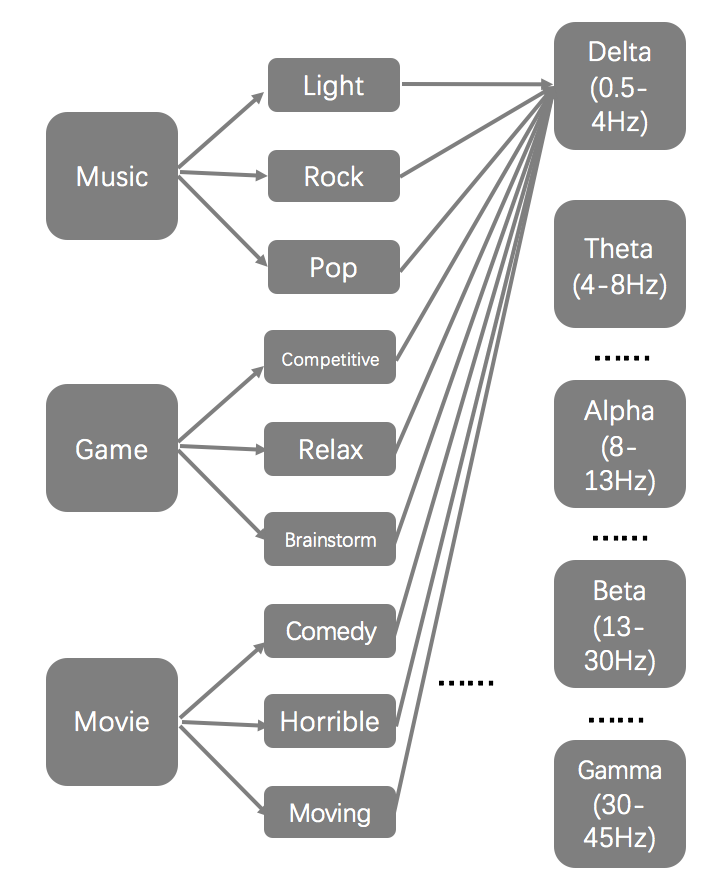
\includegraphics[width=0.6\linewidth]{fig/one-1}
  \put(-15,-30){\special{psfile = fig1.ps hscale = 100 vscale = 100}}
\end{picture}\\
  \caption{One-Way ANOVA Map.}
  \label{fig:one-1}
\end{figure}

Finally, we built the hypothesis $H_0$ is there is no emotion difference affected by different nine types of activities at the level = 0.95. The critical value goes to $F_c$=ss.f.ppf(0.95, 8, 81)=2.06 as nine types and 10 samples for each type. The results of one-way ANOVA is shown in Table 1. We can observe that each activity do has an influence on emotion in all brain wave frequency range. In the next section, we will discuss which factor has a key effect on emotion.

\begin{figure}[t]
\begin{picture}(300,150)(-10, -50)
  \centering
  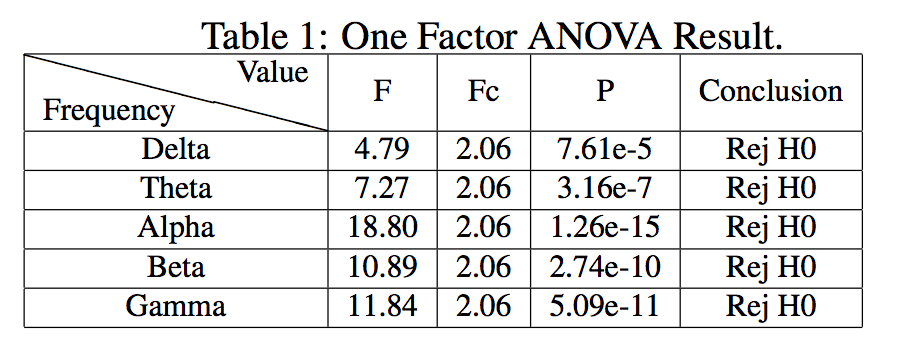
\includegraphics[width=1.0\linewidth]{fig/one-table}
  \put(-15,-30){\special{psfile = fig1.ps hscale = 100 vscale = 100}}
\end{picture}\\
  % \caption{One Factor Map.}
  \label{fig:one-table}
\end{figure}

% \begin{table}[t]
% \caption{One Factor ANOVA Result.}
% \scalebox{0.8}{
% \begin{tabular}{|c|c|c|c|c|c|}\hline
% \backslashbox{Frequency}{Value}&F&Fc&P&Conclusion\\\hline
% Delta&4.79 &2.06&7.61e-5 &Rej H0 \\\hline
% Theta&7.27 &2.06 &3.16e-7 &Rej H0\\\hline
% Alpha&18.80 &2.06 &1.26e-15 &Rej H0 \\\hline
% Beta&10.89 &2.06 &2.74e-10 &Rej H0\\\hline
% Gamma&11.84 &2.06 &5.09e-11 &Rej H0\\\hline
% \end{tabular}
% }
% \caption{One Factor ANOVA Result.}
% \label{tab:one}
% \end{table}

\subsection{Two-way ANOVA}
In this section, we conducted the Two-way ANOVA analysis. The factors we considered in this section are mobile game and music. Two levels of games, namely Player Unknown’s Battlegrounds (level 1) and Anipop (level 2) are chosen. Two levels of music, namely light music (level 1) and rock music (level 2) were selected. In this experiment, the testee played mobile game and listened to music at the same time, and the levels of music were alternated randomly, and the brain waves were recorded. The amplitude values of different band of brain waves are listed in Table 2. Each measurement was repeated three times.
\begin{figure}[t]
\begin{picture}(300,150)(-10, -10)
  \centering
  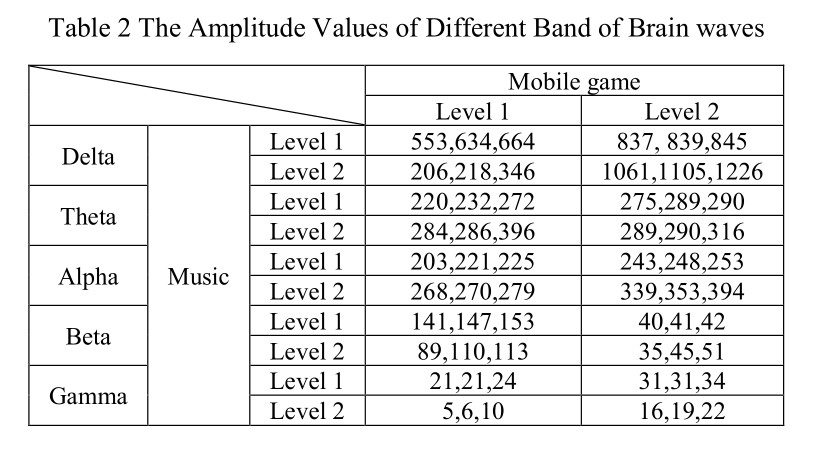
\includegraphics[width=1.0\linewidth]{fig/table2}
  \put(-15,-30){\special{psfile = fig1.ps hscale = 100 vscale = 100}}
\end{picture}\\
  % \caption{One Factor Map.}
  \label{fig:table2}
\end{figure}

Using the two-way ANOVA analysis, we obtained the variability and mean squares of the data. Here the null hypothesis is set to be $H_0$: the main effect of mobile game, main effect of music, and the interaction effect of electronic game and music are not statistically significant at $\alpha$ =0.05 level. The two-way ANOVA analysis results are given in Table 3. From the result, we can conclude that mobile game has a significant influence on Delta, Theta, Alpha and Gamma wave; music has a significant influence on Delta and Alpha wave. And the interaction has a significant effect on Delta and Gamma wave.
\begin{figure}[t]
\begin{picture}(300,150)(-10,-50)
  \centering
  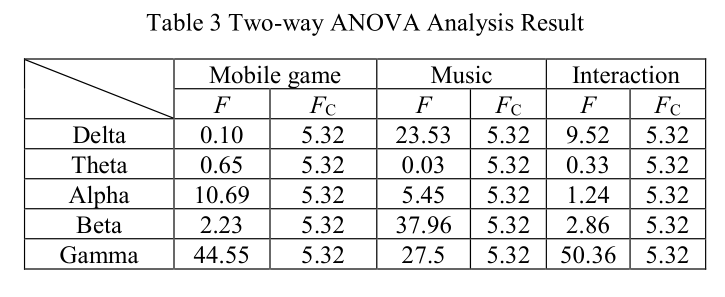
\includegraphics[width=1.0\linewidth]{fig/table3}
  \put(-15,-30){\special{psfile = fig1.ps hscale = 100 vscale = 100}}
\end{picture}\\
  % \caption{One Factor Map.}
  \label{fig:table3}
\end{figure}


\subsection{Hotteling $T^2$ Test}

As we have found that the different scenarios had discernable effects on brain activities in the previous section, multivariate Hotteling $T^2$ was implemented to further study the similarity among these scenarios.

We first chose the peace scenario as the goal. In each test, we selected the mean magnitude in each rhythm to represent the characteristic value. Each test was reduced to a five-dimension vector. Then the mean of the goal was obtained. As we set the goal, we calculated the $T^2$ with another scenario according to the formula, which tested the differentiation between these two datasets. For example, we investigated the dataset of PUBG scenario as following (Table 4).
\begin{figure}[t]
\begin{picture}(300,150)(-10,-10)
  \centering
  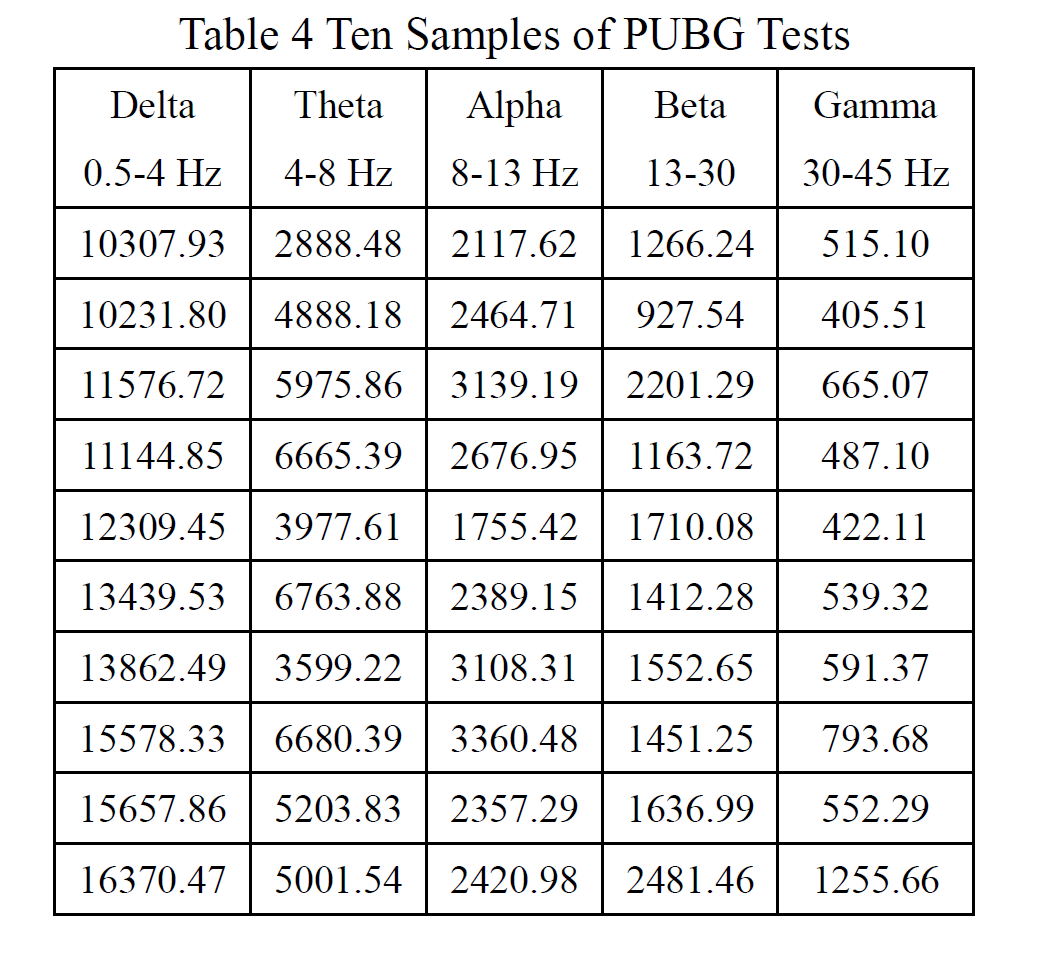
\includegraphics[width=1.0\linewidth]{fig/table4}
  \put(-15,-30){\special{psfile = fig1.ps hscale = 100 vscale = 100}}
\end{picture}\\
  % \caption{One Factor Map.}
  \label{fig:table4}
\end{figure}

The goal was [17924.43540231, 7008.93736214, 3691.29618462, 2224.2803432, 1017.29154525]. Utilizing the data above, we calculated the covariance matrix $\bm{C}$ as shown.
\begin{displaymath}
\bm{C}=\begin{bmatrix}
5204498&732140&268257&578815&393785\\
732140&1878939&303361&6006&49201\\
268257&578815&393785&303361&6006\\
49201&247631&20125&33175&20125\\
217966&87949&33175&87949&62437
\end{bmatrix}
\end{displaymath}

Thus, the calculated $T^2$ was 81.02 and the F-value was $F=9.00$. The corresponding probability was 0.98. The critical F-value for $\alpha$=0.05 was $F_{0.05}(5,5)= 5.05$. We concluded that playing PUBG would interfere with your relaxation. Similarly, we repeated the calculation to compare other eight scenarios with the peace, which resulted in a $T^2$-vector and F-vector.

$T^2=[81, 29, 511, 1167, 1192, 950, 1267, 4010, 904]$,

$F = [9, 3, 56, 129, 132, 105, 140, 445, 100]$,

According to these F values, we can see that the poker scenario did not have a significant different effect on the rhythm compared to the peace scenario at the $\alpha$=0.05 confidence level, while other scenarios had significant differences. According to testee's feedback, he is only comfortable with Poker game. He didn't try out the other game before, so he is fully intensed while playing other games.

\section{Error Discussion}
In this section, we will discuss the source of errors.

\subsection{Illegitimate Error}

Illegitimate errors come from mistakes. For example, bad or wrong observations could lead to illegitimate errors. In our experiments, there are two sources produced from illegitimate errors: one is from the testee wrong behavior like listening to music with eyes open or conducintg other activities, the other is we collected data without AC in the off-state and one additional 50Hz disturbation was generated.

\subsection{System Error}

In our experiment, system errors can result from as follow: the tested position of brain and the equipment calibration. Currently we only have two input probing and one reference probing to collect data. There is other more precise device for EEG electrode positions is the placement of 21 electrodes. Another system error is that equipment sometimes collected the time and volts data in the wrong format. For example, it only return time without volts. Sometimes it leads to interruption of data parsing process.

\subsection{Statistical Error}

In our research experiment, the statistical error result from two areas: one is the data collection period. We could obtain more rich brain wave data by extending the collection time (i.e., measure result from 1 min, 10 mins and even longer time). Another can be addressed to the sample size. Because we chose totally 9 activities to do the analysis, we collected 10 to 20 samples data for each activity. We are looking forward to testing more samples to improve the accuracy of results in the future.


\section{Conclusions}
In this project, we used several statistical technologies to analyze the brain behavior. The brain waves were obtained by the EEG collector. Then the fast Fourier transform was utilized to transform the time domain waveform into frequency domain. After filtering, the delta, theta, alpha, beta and gamma waves were extracted. By analyzing the amplitude in the frequency domain using one-way ANOVA, Hotteling $T^2$ and two-way ANOVA test, we identified the significant contributors to the changing of brain waves when doing different activities like playing mobile games, watching movies and listening to music. The result we obtained could be a potential guidance to help us to adjust the brain waves by doing these daily activities according to indiviual behaviour. For example, we found that playing poker results in a similar brave wave pattern with the silence state. Future works include reducing the fluctuation of the measurement and introducing more complex statistic model to improve the accuracy in obtaining the influence from each factors.

{\normalsize
\bibliographystyle{unsrt}
% \bibliographystyle{acm}
\bibliography{usenix}}


% \theendnotes
\end{document}
